
\chapter{Tested Algorithms}
\label{TestedAlgorithms}
In this chapter we present some of the results performed for simple
real-valued genetic algorithms which were tuned for benchmark
functions (see next section).
As an embedded EA we have used a genetic
algorithm with real-encoding, proportionate selection and genetic operators 
based on normal distribution.

\section{Benchmark functions}
Tests were performed for simple, multimodal, two dimensional functions:
\begin{itemize}
  \item $f(X) = 2e^{-((x+1.1)^2 + (y+1.1)^2)} + 1.5e^{-((x-1)^2 + y^2)} +
  4e^{-3((x+1.5)^2 + (y-1.5)^2)}$, where $X \in \mathbb{R}^2$
  \item $f(X) = e^{-(x^2 + y^2)}+1.4e^{-((x-1.7)^2 + (y-1.7)^2)}$, where $X \in
  \mathbb{R}^2$
\end{itemize} 

\section{Tests}
\begin{figure}
  \centering
  \fbox{
    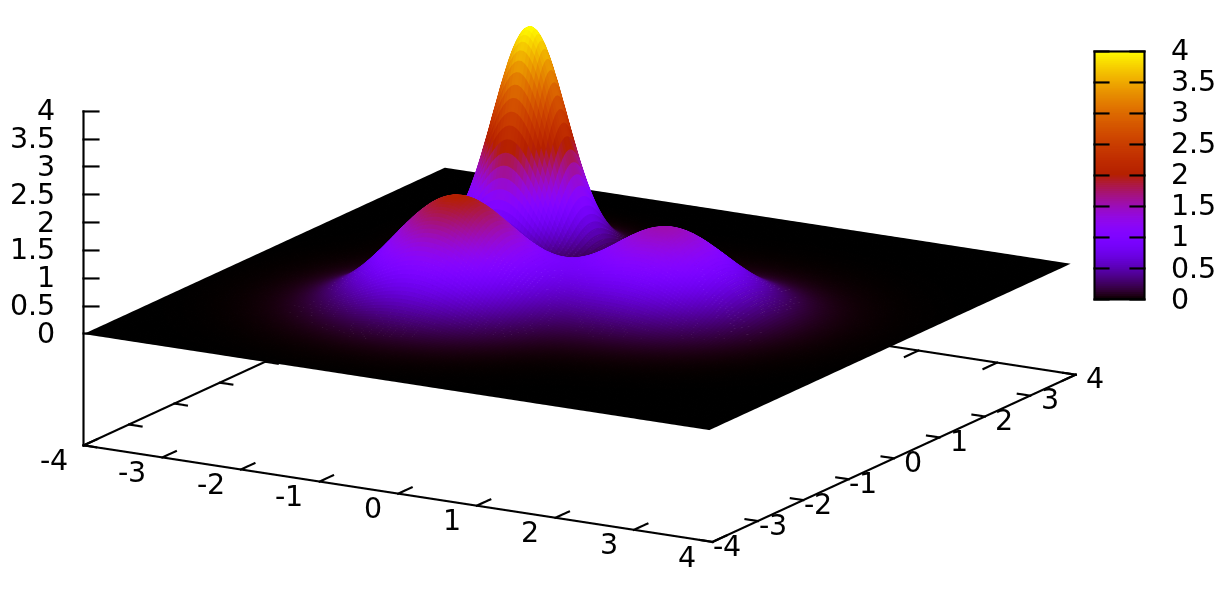
\includegraphics[scale=0.2]{weighted_1_0/ofl1.png}
  }
  \fbox{
    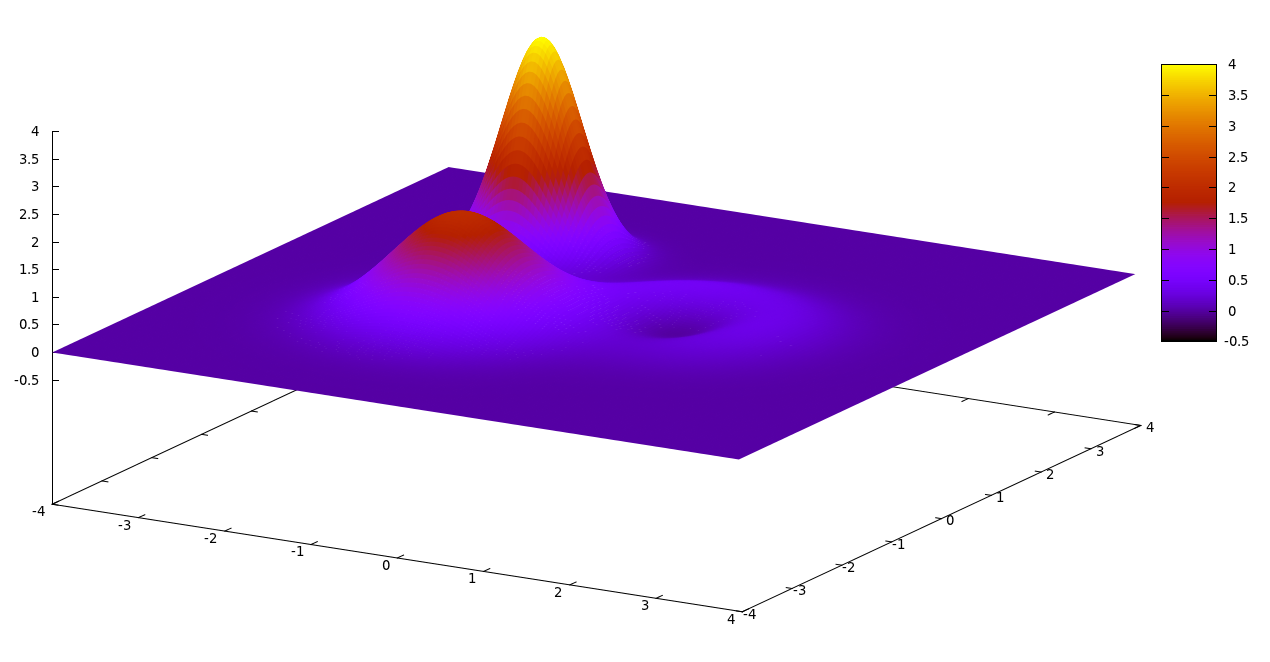
\includegraphics[scale=0.2]{weighted_1_0/iter11.png}
  }
  \fbox{
    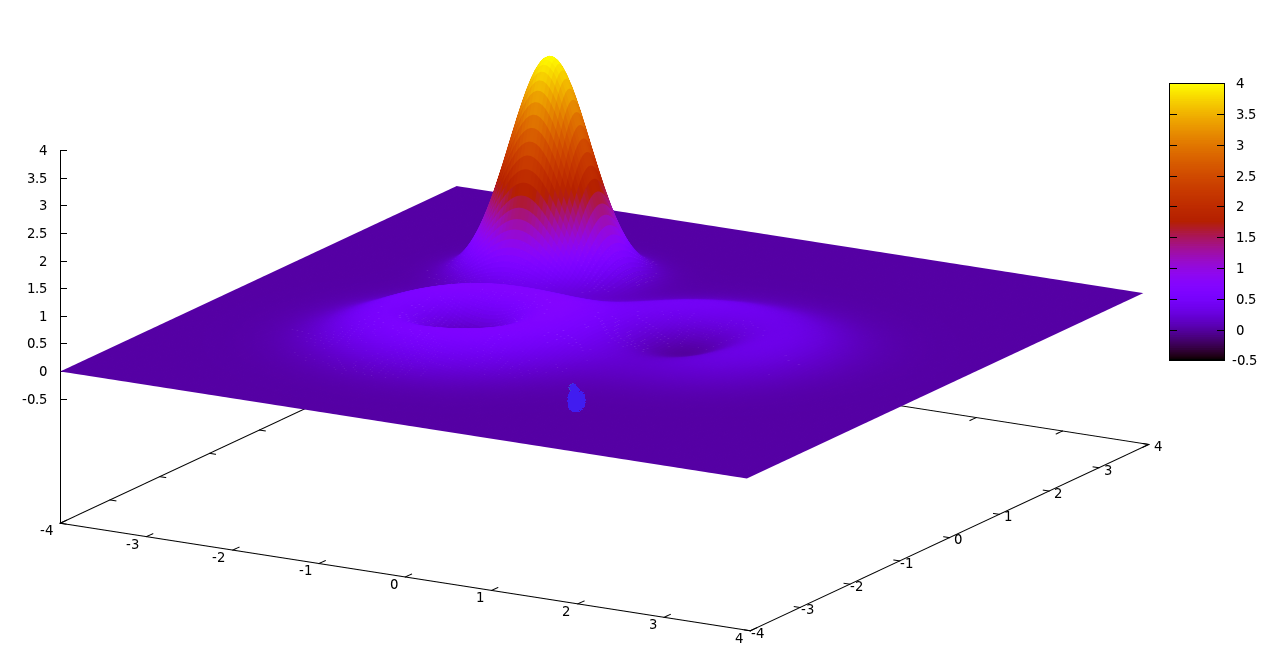
\includegraphics[scale=0.2]{weighted_1_0/iter12.png}
  }
  \fbox{
    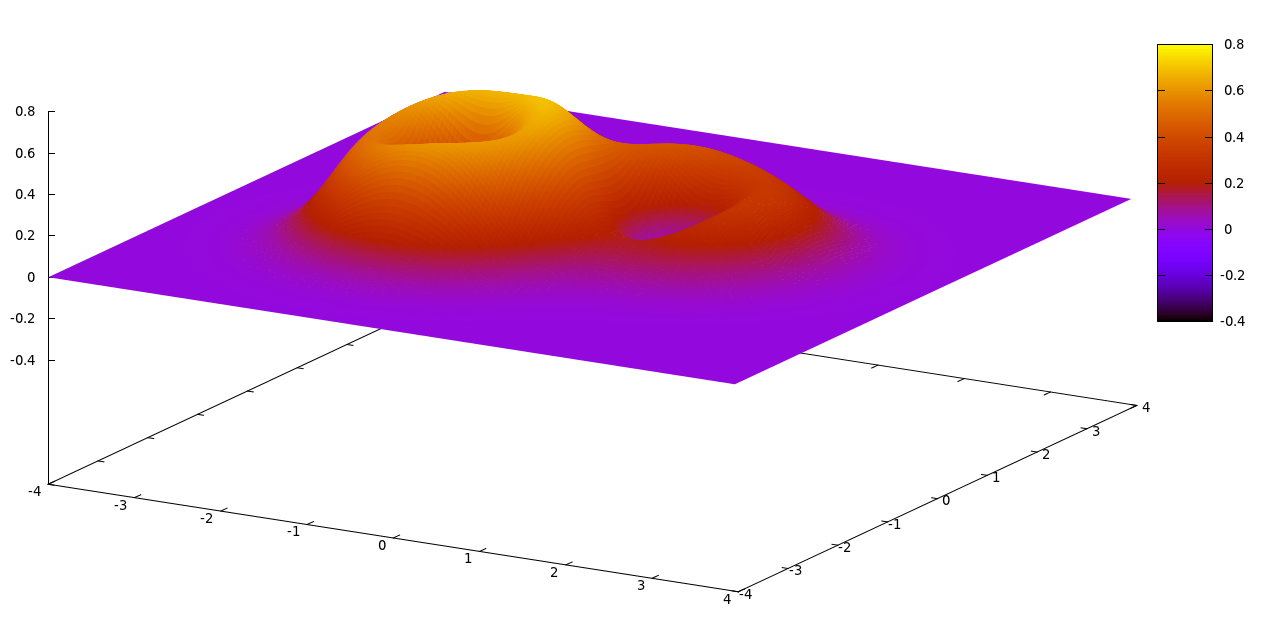
\includegraphics[scale=0.2]{weighted_1_0/iter13.png}
  }
  \caption{The result of sequential niching algorithm applied for the function:
  $f(X) = 2e^{-((x+1.1)^2 + (y+1.1)^2)} + 1.5e^{-((x-1)^2 + y^2)} +
  4e^{-3((x+1.5)^2 + (y-1.5)^2)}$. OPTICS parameters: $\epsilon=0.5,
  minPts=10$, deterioration algorithm: \textit{Weighted scheme}}
  \label{seqNiching1}
\end{figure}

\begin{figure}
  \centering
  \fbox{
    \includegraphics[scale=0.3]{weighted_1_0/pop_pm3d11.png}
  }
  \fbox{
    \includegraphics[scale=0.3]{weighted_1_0/pop_pm3d12.png}
  }
  \fbox{
    \includegraphics[scale=0.3]{weighted_1_0/pop_pm3d13.png}
  }
  \caption{Clusters returned in subsequent interations of sequential
  niching algorithm applied for function
  $f(X) = 2e^{-((x+1.1)^2 + (y+1.1)^2)} + 1.5e^{-((x-1)^2 + y^2)} +
  4e^{-3((x+1.5)^2 + (y-1.5)^2)}$. The resulted fitness function is visualized 
  as a color map (\textit{pm3d}). We have found all solutions and achieved
  $80\%$ of the overall fitness landscape decline}
  \label{seqNichingPop}
\end{figure}

\begin{figure}
  \centering
  \fbox{
    \includegraphics[scale=0.3]{simple1/pop_pm3d11.png}
  }
  \fbox{
    \includegraphics[scale=0.3]{simple1/pop_pm3d12.png}
  }
  \fbox{
    \includegraphics[scale=0.3]{simple1/pop_pm3d13.png}
  }
  \caption{Visualization of the fitness deterioration outcomes in subsequent
  iterations. Test function: $f(X) = 2e^{-((x+1.1)^2 + (y+1.1)^2)} + 1.5e^{-((x-1)^2 + y^2)} +
  4e^{-3((x+1.5)^2 + (y-1.5)^2)}$. Deterioration algorithm: \textit{Basic
  scheme}. We have found all solutions and achieved $85\%$ of the overall
  fitness landscape decline}
  \label{seqNichingPop}
\end{figure}





